\documentclass{article}

% {{{ Preamble 
\usepackage[]{amsthm} 
\usepackage[]{amsmath} 
\usepackage[]{amssymb} 
\usepackage[]{thmtools} 

\usepackage[]{fontspec} 

% Code listings
\usepackage[]{listings}
\usepackage[usenames, dvipsnames, svgnames, table]{xcolor}
\usepackage[]{mdframed}
\usepackage[]{calc} 

\definecolor{TMcodeBackground}{RGB}{224, 224, 224}
\definecolor{TMcodeFrame}{RGB}{109, 108, 109}
\definecolor{TMgreen}{RGB}{14, 191, 48}
\definecolor{TMorange}{RGB}{243, 126, 25}
\definecolor{TMred}{RGB}{230, 6, 85}

\defaultfontfeatures{Ligatures=TeX}
\setmonofont{Source Code Pro Light}[BoldFont=Source Code Pro]

\mdfdefinestyle{TMstyleCode}{
            skipabove=4mm,
            skipbelow=0mm,
            %remove borders
            rightline=false,
            topline=false,
            bottomline=false,
            linewidth=1mm,
            %margins
            innertopmargin=2mm,
            innerleftmargin=0mm,
            innerbottommargin=0mm,
            innerrightmargin=10pt,
            linecolor=TMcodeFrame,
            backgroundcolor=TMcodeBackground
}

\lstdefinestyle{TMstyle}{
    showstringspaces=false,
    numbers=left,
    numbersep=7mm,
    numberstyle=\color{Black},
    stepnumber=1,
    tabsize=3,
    breakatwhitespace=false,
    breaklines=true,
    captionpos=b,
    basicstyle=\color{Black}\ttfamily,
    commentstyle=\color{TMgreen}\ttfamily,
    keywordstyle=\color{TMorange}\bfseries,
    stringstyle=\color{TMred},
    frame=leftline,
    framesep=0mm,
    xleftmargin=3mm,
    framesep=2mm,
    framerule=0mm,
    abovecaptionskip=5mm,
    aboveskip=\baselineskip,
    belowskip=\baselineskip
}

\lstnewenvironment{TMcode}[3]
{
    \lstset{style=TMstyle, language=#1, caption=#2}
    \mdfsetup{style=TMstyleCode}
    \mdframed
    \hspace*{3mm}
    \minipage{0.75cm}
    
\includegraphics[width=\linewidth]{../pictures/code2.png}
    \endminipage
    \hspace*{1mm}
    \minipage{\textwidth-1.05cm}
        {\sffamily\Large #3}
    \endminipage
    \vspace*{-2mm}
}
{
    \endmdframed
}

\usepackage[]{graphicx} 
\usepackage[]{subcaption} 

\declaretheorem[style=definition,qed=$\clubsuit$]{definition}
\declaretheorem[style=definition,qed=$\spadesuit$,sibling=definition]{example}
\declaretheorem[style=definition,qed=$\diamondsuit$]{corollary}
\usepackage[margin=2cm]{geometry} 

\usepackage[]{url} 
\urlstyle{sf}
\usepackage[]{makeidx} 
\makeindex
\usepackage[]{cleveref} 

\newcommand{\R}{\mathbb{R}}
\newcommand{\C}{\mathbb{C}}
\newcommand{\A}{\mathbb{A}}
\newcommand{\V}{\mathbb{V}}
\newcommand{\Bu}[2]{\mathrm{Bl}_{#1}\A^{#2}}
\renewcommand{\P}{\mathbb{P}}

\DeclareMathOperator{\rank}{rank}
\DeclareMathOperator{\col}{Col}
% }}}

\title{Algebraic Surfaces}
\author{Ivar Haugal{\o}kken Stangeby}
\date{MAT2000 --- Spring 2016}

\begin{document}
\maketitle    

\begin{abstract}
    In this paper we take a closer look at algebraic surfaces. With an emphasis
    on the visual aspects we look at singularities of surfaces, their
    symmetries, as well as techniques for resolving singularities. Unless
    specificed, the images are rendered in the software \textsc{Surfer}.
\end{abstract}

\tableofcontents

\section{Preliminaries}
\label{sec:preliminaries}

In algebraic geometry the objects of study are, amongst other, the set of
solutions to polynomial equations. Finding the zeroes of a quadratic equation
\begin{equation}
    \notag
    ax^2 + bx + c = 0
\end{equation} 
is something most people who have been exposed to elementary mathematics have
done. Later one learns how to find the zeroes of more general functions $f \in
K[x_1, x_2, \ldots, x_n]$ of either one or several variables, and you often
find functions that have no zeroes at all. 

One of the central objects in algebraic geometry is the \emph{affine algebraic
variety}\index{variety!affine algebraic variety} and the \emph{projective
variety}\index{variety!projective variety}. These are defined as the set of
common solutions to the zero-equations of a set of polynomials in some
\emph{polynomial ring}\index{polynomial ring}.

\begin{definition}[Polynomial ring]
    A \emph{polynomial ring} in $n$ variables $K[x_1, x_2, \ldots, x_{n}]$ over a
    field $K$ is the set of all functions on the form
    \begin{equation}
        \notag
        f(x) = \sum_{\alpha} p_\alpha \prod_{i=1}^{n} x_n^{\alpha_i}
    \end{equation}
    where $\alpha = (\alpha_1, \ldots, \alpha_n)$ is a multi-index and
    $p_\alpha = p_{\alpha_1\ldots\alpha_n}$ is a coefficient in $K$.
\end{definition}
An example of a polynomial ring is $\R[x, y]$. Elements include $f_1(x, y) =
x^2y + y + 1$ and $f_2(x, y) = \pi$. Given a set of polynomials $\left\{f_1, f_2, \ldots,
f_m\right\}$ in a polynomial ring $K \left[ x_1, x_2, \ldots, x_n \right]$ we can look at
their common zeroes. Specifically for polynomials in \emph{affine space}\index{space!affine} we
make the following definition.

\begin{definition}[Affine algebraic variety]
    Given a set of polynomials $\left\{ f_1, f_2, \ldots, f_m \right\}$ from a ring
    of polynomials, the set of points $(x_1, x_2, \ldots, x_n)$ in the affine space
    $\A^n$ that satisfy
    \begin{equation}
        \notag
        f_i(x_1, \ldots, x_n) = 0 \quad \text{for} \quad i = 1, \ldots, m
    \end{equation}
    is called an \emph{affine algebraic variety} and is denoted $\V(f_1, f_2,
    \ldots, f_m)$.
\end{definition}

Given the polynomial $f(x) = x^2 - 1$, the affine algebraic variety $\V(f)$ is
then the set of points $\left\{ 1, -1 \right\}$ since $f(-1) = f(1) = 0$.
Given an additional polynomial $g(x) = x-1$ we have $\V(f, g) = \left\{ 1
\right\}$. Finally, if we also consider the polynomial $h(x) = x^2$, then
$\V(f, g, h) = \emptyset$. We therefore see that the variety of a set of
function is an intersection of the varieties of the individual functions.

In this paper we will also deal a lot with singularities of our algebraic
surfaces. We make a formal definition.
\begin{definition}[Singularity]
    A singularity of the variety $V = \V(f_1, f_2, \ldots, f_m)$ is a point $p$ such
    that the Jacobian matrix
    \begin{equation}
        \notag
        \begin{bmatrix}
            \frac{\partial f_1}{\partial x_1} && \hdots && \frac{\partial f_1}{\partial x_n} \\
            \vdots && \ddots && \vdots \\
            \frac{\partial f_m}{\partial x_1} && \hdots && \frac{\partial f_m}{\partial x_n}
        \end{bmatrix}(p)
    \end{equation} has rank strictly less than $\min(m, n)$.
\end{definition}

A very useful consequence of this definition deal with varieties of single
polynomials.
\begin{corollary}
    \label{crl:single_poly}
    A point $p$ is a singularity of the variety $\V(f)$ if and only if the
    partial derivatives of $f$ vanish identically at $p$. Mathematically this
    is expressed as ${\partial f(p)}/{\partial x_i} = 0$ for $i = 1, 2, \ldots,
    n$.
\end{corollary}
\begin{proof}
    We recall that the \emph{rank}\index{rank} of a matrix $A$ is the dimension of its
    column space. Note that $\min(m, n)$ is in this case equal to $1$ since we
    have $n$ variables but only one function.
    For the Jacobian matrix
    \begin{equation}
        \notag
        A = \begin{bmatrix}
            \frac{\partial f_1}{\partial x_1} && \hdots && \frac{\partial f_1}{\partial x_n}
        \end{bmatrix}(p)
    \end{equation} 
    to have rank strictly less then one, its column space has to have dimension
    zero. In linear algebra terms, this simply means that the matrix have no
    pivot columns, and hence each column must be zero. Therefore, for $p$ to be
    a singularity of $\V(f)$ all its partial derivatives must vanish
    identically.
\end{proof}


\section{Algebraic Surfaces}
\label{sec:algebraic_surfaces}

In this section we try to motivate the definition of an algebraic surface and
look at some examples, and hopefully give an intuitive explanation of what
exactly we are looking at. Looking at real algebraic curves is a good entry
point.

\subsection{An Informal Introduction}
\label{sub:an_informal_introduction}

From elementary mathematics one learns about real valued functions, $f(x)$, and
how to graph these functions by setting $y = f(x)$ and plotting points in the
$(x, y)$-plane. Now, the \emph{graph of a function}\index{graph} is something of a
pecuiliarity, because it comes with some restrictions. Not all curves in the
$(x, y)$-plane correspond to a specific function. The method for verifying
whether a certain ''graph'' correspond to a function or not, typically taught
in school, is the \emph{vertical line test}. 

Having an equation $y = f(x)$ we can form what we call the \emph{equation of a
curve at zero}\index{equation at zero}. We define a new function in two variables
\begin{equation}
    \notag
    g(x, y) = y - f(x) = 0.
\end{equation}
If the function $f(x)$ is a polynomial in the variable $x$ we call the function
graph of $f(x)$ \emph{algebraic}. If the distinction between a graph and a
curve is to be justified there has to be some curves that are not graphs. If we
look at what happens when you set $y^2 = x^3$, then the plotted curve does not
pass the vertical line test, and is therefore something different from a
function graph. Similarily, the equation $y^2 = x^3 - x^2$ defines a curve that
is again not a graph. These curves also happen to exhibit \emph{singular
points}\index{singular point} at $(0, 0)$.

With what we have so far, we can move up a dimension. Instead of considering
curves in the $(x, y)$-plane we can look at surfaces in $(x, y, z)$-space.
Following the same procedure as above, we define a new function $h(x, y, z) = z
- g(x, y)$. The surfaces are given by equations on the form $h(x, y, z) = 0$.
These surfaces are \emph{algebraic}\index{surface!algebraic surface} if $h(x,
y, z)$ is a polynomial in the variables $x, y, z$. 

\begin{example}
    \label{exmpl:algebraic_surfaces}
    The following equations satisfy the definition of an algebraic surface
    \begin{enumerate}
        \item $h_1(x, y, z) = z - xy = 0$,
        \item $h_2(x, y, z) = z - x^2 - y^2 = 0$,
        \item $h_3(x, y, z) = z - (2x^2-y)(y-x^2)$,
    \end{enumerate}
    where as the following does not satisfy the definition:
    \begin{enumerate}
        \item $g_1(x, y, z) = \sin(xy) + z$,
        \item $g_2(x, y, z) = \tan^2(x) + \pi zy$.
    \end{enumerate}
    The examples of algebraic surfaces are shown visualized in
    \cref{fig:algebraic_surfaces}.

    \begin{figure}[]
        \centering
        \begin{subfigure}[t]{0.3\textwidth}
            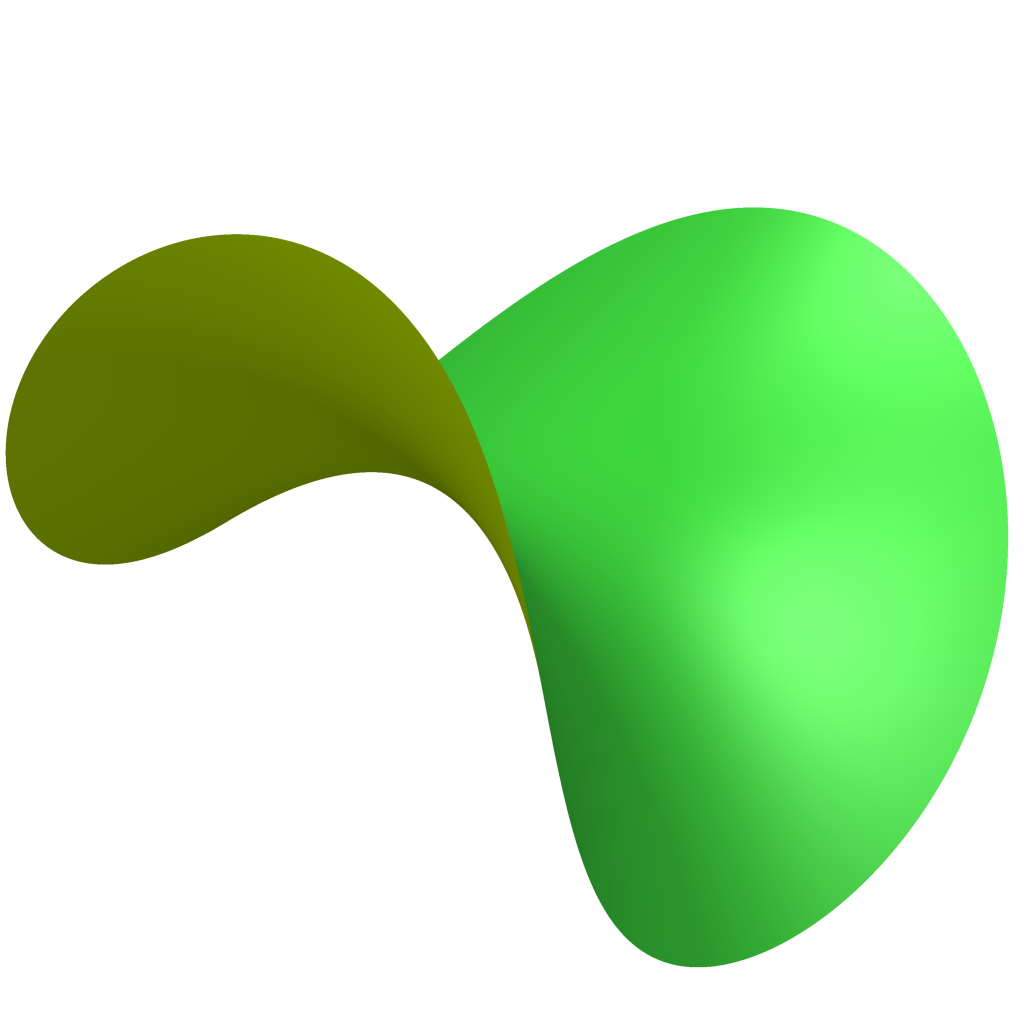
\includegraphics[height=0.6\textwidth, width=0.6\textwidth]{../pictures/example_one.png}
            \caption{$h_1(x, y, z) = 0$.}
        \end{subfigure}
        ~
        \begin{subfigure}[t]{0.3\textwidth}
            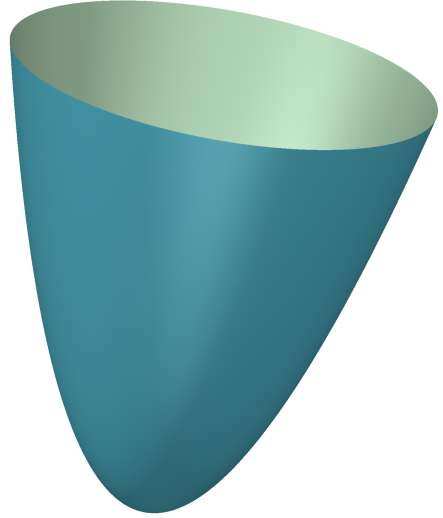
\includegraphics[height=0.6\textwidth, width=0.6\textwidth]{../pictures/example_two.png}
            \caption{$h_2(x, y, z) = 0$.}
        \end{subfigure}
        ~
        \begin{subfigure}[t]{0.3\textwidth}
            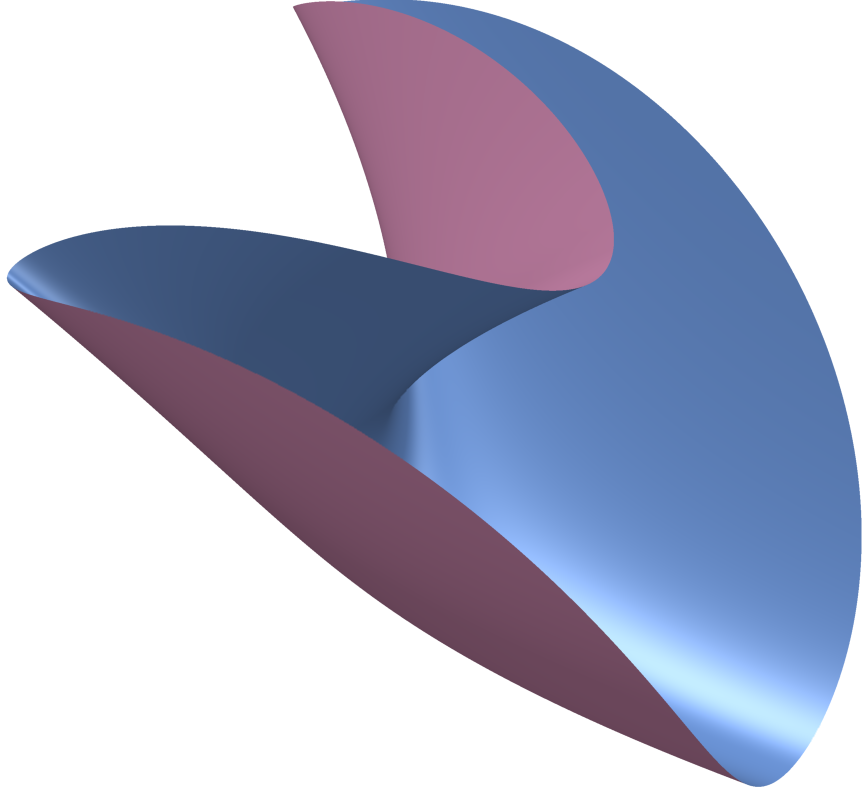
\includegraphics[height=0.6\textwidth, width=0.6\textwidth]{../pictures/example_three.png}
            \caption{$h_3(x, y, z) = 0$.}
        \end{subfigure}
        \caption{The algebraic surfaces from \cref{exmpl:algebraic_surfaces}.}
        \label{fig:algebraic_surfaces}
    \end{figure}
\end{example}

We complete this section by formally defining an algebraic surface.
\begin{definition}[Algebraic surface]
    An \emph{algebraic surface}\index{surface!algebraic surface} is an
    algebraic variety of dimension two.\footnote{The dimension of an algebraic
    variety is a bit hard to grasp, and since we only will deal with
    algebraic surfaces in this article we do not spend any time classifying
    the different kinds of varieties.}

    We define the \emph{degree}\index{surface!degree} of the algebraic surface
    to be highest combined power in the defining polynomials terms, and denote
    this $d$, i.e.,
    \begin{equation}
        \notag
        d = \max_{\alpha}\left\{\alpha_1 + \alpha_2 + \ldots + \alpha_n\right\}
    \end{equation}
    where the $\alpha_i$ is the power of $x_i$ in a term.
\end{definition}


\section{Singularities}
\label{sec:singularities}

The singularities of an algebraic surface is one of the more important elements
that give the surfaces its visual appeal. I am sure many people would agree
with me that surfaces with many singularities, and with singularities in
interesting configurations, are more exciting to look at then the surfaces that
show no singularities. 

We first take a look at the number of singularities that various surfaces have.

\subsection{The Number of Singularities}
\label{sub:the_number_of_singularities}

For an algebraic surface of degree $d$ we let $\mu(d)$ denote the maximum
number of singularities such a surface \emph{can} exhibit. We first look at
some examples that help illustrate this.

\begin{example}[The plane has no singularities]
    The defining polynomial of a plane in three dimensions is 
    \begin{equation}
        \notag
        f(x, y, z) = ax + by + cz + d.
    \end{equation}
    The corresponding surface is then $V = \V(f)$. We want to find the
    singularities of $V$. Applying \cref{crl:single_poly} we only need consider
    the partial derivatives and find the points in $V$ where they vanish. We
    solve the equations
    \begin{align*}
        \frac{\partial f}{\partial x} = \frac{\partial f}{\partial y} = \frac{\partial f}{\partial z} = 0.
    \end{align*} 
    This gives $a = 0$, $b = 0$ and $c = 0$ which again forces $d = 0$ since
    otherwise our point $(x, y, z)$ would not be a zero of $f$. This however,
    tells us that $f(x, y, z) = 0$ which does not define any surface. Hence,
    the plane has no singularities. The plane is an algebraic surface of degree
    $d = 1$, so consequently $\mu(1) = 0$.
\end{example}

\begin{example}[The Cayley cubic]
    The Cayley cubic is defined by the polynomial
    \begin{equation}
        \notag
        f(x, y, z) = xyz + (1 - x - y - z)(yz + xz + xy).
    \end{equation}
    Again, we are interested in the singularities of $V = \V(f)$. Once again,
    we apply \cref{crl:single_poly} and look at the partial derivatives and
    find their zeroes. This gives the four points $(0, 0, 0)$, $(0, 0, 1)$,
    $(0, 1, 0)$ and $(1, 0, 0)$.

    It can also be shown that there cannot be \emph{more} than four
    singularities for a third degree surface. Hence $\mu(3) = 4$.
\end{example}

\subsection{Symmetric Singularities}
\label{sub:symmetric_singularities}


\section{Resolving Singularities}
\label{sec:resolving_singularities}

We call a variety that exhibits no singularities \emph{smooth}\index{smooth}.
It is often possible to study a smooth copy of a variety with singularities if
we move from affine space to projective space.

\subsection{Projective Space}
\label{sub:projective_space}

In this section we define the notion of a \emph{projective
space}\index{space!projective}.  Informally, projective space formalizes the
notion of parallel lines intersecting at infinity.

The general definition of projective $n$ space is the set of lines in
$\C^{n+1}$ passing through the origin.
\begin{definition}[The projective space of dimension $n$]
    Let $\sim$ be an equivalence relation on $\C^{n+1} \setminus 0$ defined by
    \begin{equation}
        \notag
        \left( x_1, \ldots, x_{n+1} \right) \sim \left( x_1', \ldots,
        x_{n+1}' \right) \iff \left( x_1', \ldots, x_{n+1}' \right) =
        \lambda \left( x_1, \ldots, x_{n+1} \right)
    \end{equation}
    where $\lambda$ is some non-zero complex number. We denote the equivalence
    class of $\left( x_1, \ldots, x_{n+1} \right)$ by $\left[ x_1 : \ldots :
    x_{n+1} \right]$ and define the \emph{projective space of dimension $n$} as
    the set
    \begin{equation}
        \notag
        \P^n{\C} = \left\{ \left[ x_1 : \ldots : x_{n+1} \right] \mid
        \left( x_1, \ldots, x_{n+1} \right) \in \C^{n+1} \setminus
        0 \right\}.
    \end{equation}
\end{definition}
\subsection{Blowups}
\label{sub:blowups}

Informally, when we blow up a point $p$ in $\A^n$, we replace the point $p$ by
an entire copy of a projective space $\P^{n-1}$ and try to leave the rest of
the space $\A^n$ unchanged. We will give a few examples of this.

\begin{definition}[Blowup of $\A^n$ at $p$]\index{blowup!point}
    \label{defn:blowup_point}
    We let the blowup-surface\index{surface!blowup} $\Bu{p}{n}$ be the set of all
    pairs consisting of a point $p
    \in \A^n$ and a line from $p$ through the origin.  Then $\Bu{p}{n} \subseteq
   \A^n\times\P^{n-1}$. We write
   \begin{align*}
       \notag
       \Bu{p}{n} &= \left\{ (p, L) \mid p \in \A^n, p \in L \right\} \\
         &= \left\{ (x_1, \ldots, x_n ; y_1: y_2: \ldots :y_n) \mid x_iy_j =
           x_jy_i \quad 0 \leq i < j \leq n \right\}.
   \end{align*}
\end{definition}

In order to aid us with this, we have the following result:
\begin{corollary}
    \label{crl:minors}
    Given a point $x = (x_1, \ldots, x_n)$ in the space $\A^n$ and a point $y =
    \left( y_1 : \ldots : y_n \right)$ in the space $\P^{n-1}$ the point
    $x$ is a multiple of $y$ if and only if the matrix
    \begin{equation}
        \notag
        A = 
        \begin{bmatrix}
            x_1 & x_2 & \hdots & x_n \\
            y_1 & y_2 & \hdots & y_n
        \end{bmatrix}
    \end{equation}
    has rank less than or equal to one. Similarly, the rank is less than or
    equal to one only if each $2\times2$-minor $x_iy_j - x_jy_i =
    0$.\footnote{Figure this out properly.}
\end{corollary}
\begin{proof}
    In order to verify this, we recall that $\rank(A) = \rank(A^T)$, so we
    chose to work with the transposed matrix instead. Assume that $x$ is a
    multiple of $y$, so $y = \lambda x$ for some scalar $\lambda$.  Then
    \begin{align*}
        A^T = \begin{bmatrix}
            x_1 & \lambda x_1 \\
            \vdots & \vdots \\
            x_n & \lambda x_n
        \end{bmatrix}.
    \end{align*}
    Assume that the point $x$ is non-zero. Then we have exactly one pivot
    column in this matrix, hence $\dim(\col(A^T)) = 1$. If $x = 0$, then we have
    no pivot columns, so $\dim(\col(A^T)) = 0$. In any case, $\rank(A) =
    \rank(A^T) \leq 1$.

    For the second claim, since $A^T$ has rank 1, there cannot exists any
    non-zero minors $r\times r$ for $r > 1$. Hence all $2\times 2$ minors must
    vanish.
\end{proof}

\begin{example}[The Node]
    The defining polynomial of the node is given by
    \begin{equation}
        \label{eq:node}
        f(x, y) = y^2 - x^2 - x^3,
    \end{equation}
    so the curve is $C = \V(f)$. This curve lives in the affine plane $\A^2$.
    The blow-up $B_p$ of $C$ at the point $p = (0, 0)$ lives in $\A^2 \times
    \P^1$. For a point $(x, y) \in C$ we figure out what line it passes through
    by applying \cref{crl:minors} with homogeneous coordinates $(r, s)$.
    \begin{equation}
        \notag
        \begin{bmatrix}
            x & y \\
            r & s
        \end{bmatrix}
    \end{equation}
    has rank less than or equal to one when $xs - yr = 0$ (our only
    $2\times2$-minor in this case). This gives $xs = yr$. Since $r$ and $s$ are
    homogeneous coordinates, we have $(r : s) = (1 : s)$ and $(r : s) = (r :
    1)$. We can therefore eliminate either $r$ or $s$ in our equation.

    \begin{description}
        \item[Case 1] Setting $s = 1$ we get $x = yr$. Eliminating $x$ from
            \cref{eq:node} gives a new equation $g(y, r) = y^2 - y^2r^2 -
            y^3r^3 = y^2(1 - r^2 - yr^3)$. This can be visualized in the $(y,
            r)$-plane.
        \item[Case 2] Setting $r = 1$ we get $y = xs$. We can now eliminate $y$
            from \cref{eq:node} which gives another new equation $h(x, s) =
            x^2s^2 - x^2 - x^3 = x^2(s^2 - 1 - x)$ which can be visualized in
            the $(x, s)$-plane.
    \end{description}
    \begin{figure}[h!]
        \centering
        \begin{subfigure}[t]{0.3\textwidth}
            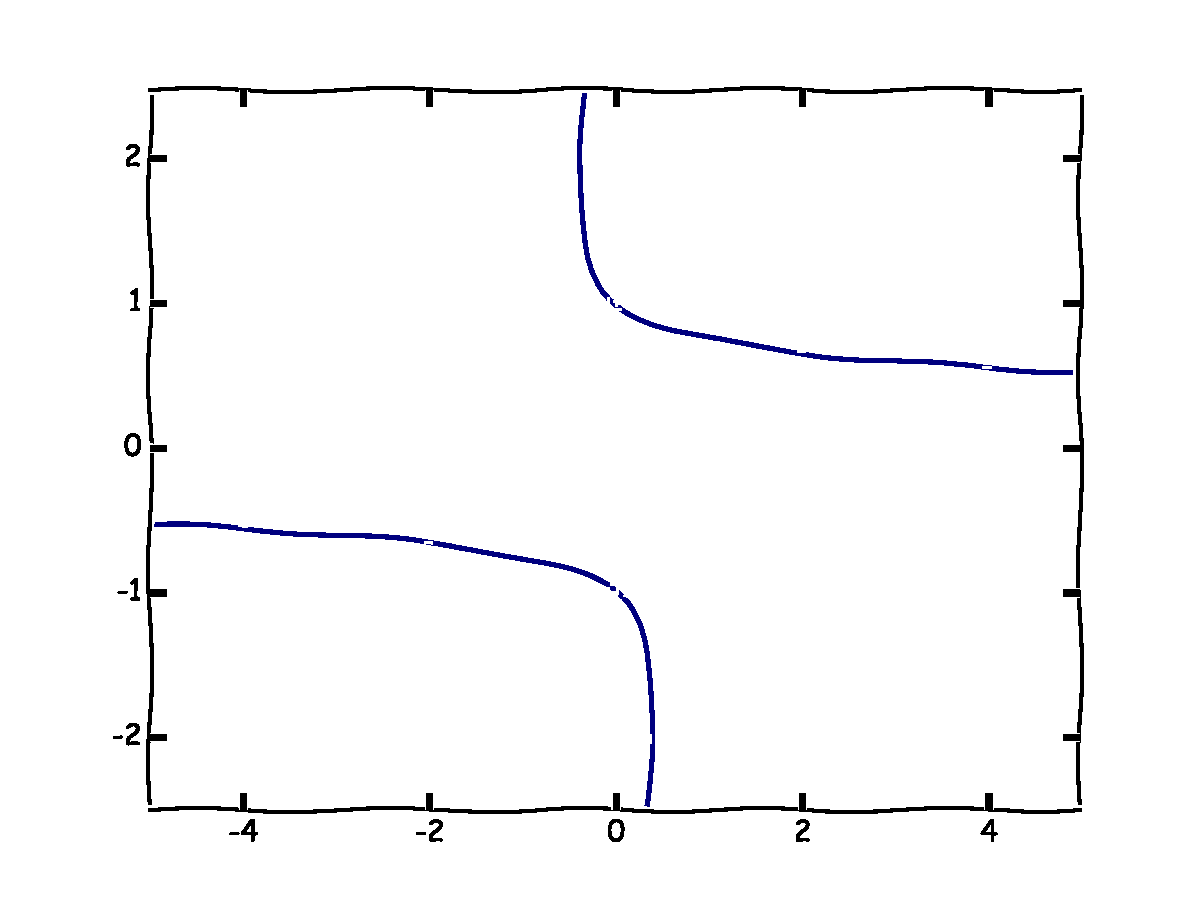
\includegraphics[width=\textwidth]{../pictures/case_1.pdf} 
            \caption{The function $g$ visualized in the $(y, r)$-plane.}
        \end{subfigure}
        ~
        \begin{subfigure}[t]{0.3\textwidth}
            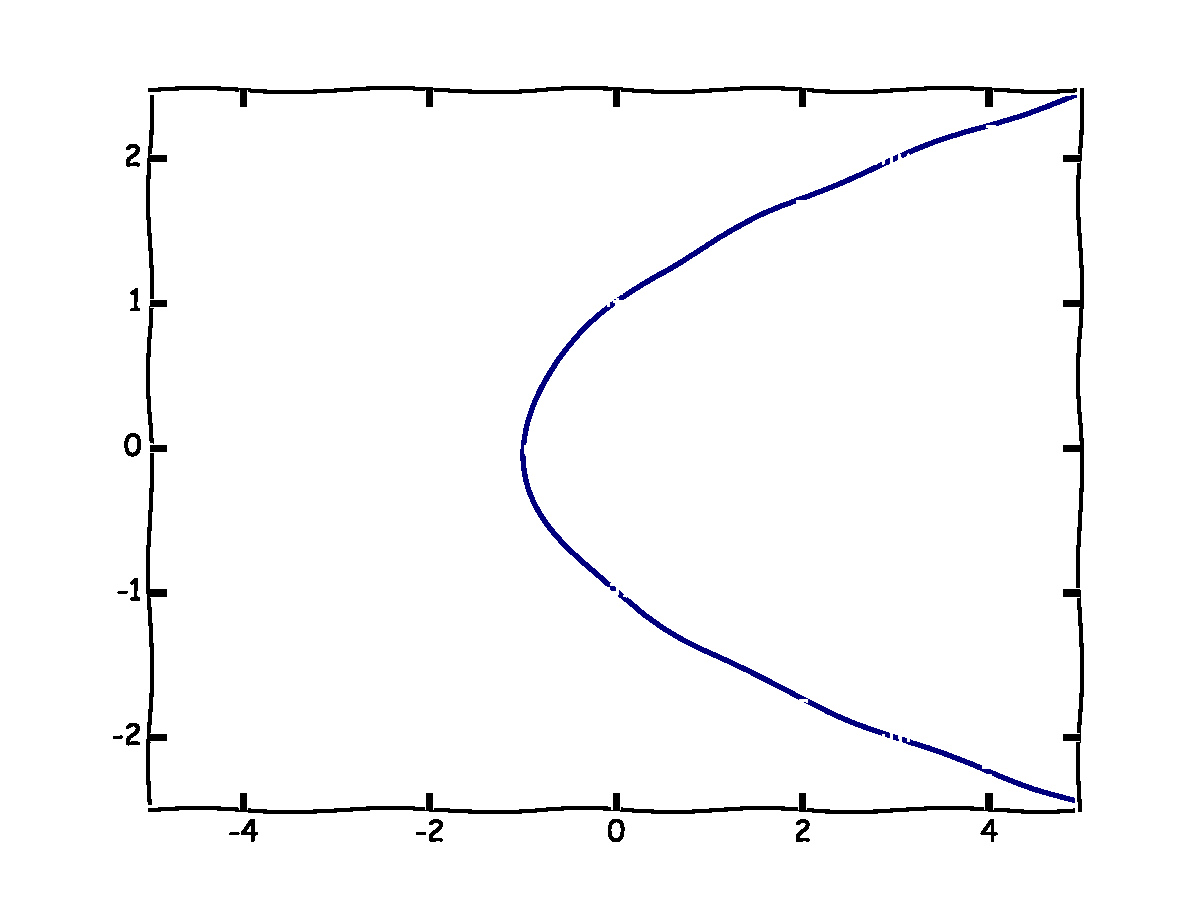
\includegraphics[width=\textwidth]{../pictures/case_2.pdf} 
            \caption{The function $h$ visualized in the $(x, s)$-plane.}
        \end{subfigure}
        \caption{The affine charts of the blow-up. Note that each of the curves
        intersect the line vertical axis twice. This corresponds to the two
        singularities of the original curve.}
    \end{figure}
    Note that the functions $g$ and $h$ are homogeneous functions, in the sense
    that $x$ and $y$ are regarded as constant and are therefore of degree
    zero.\footnote{Figure out why.} It is now of interest to see how these
    \emph{affine charts} relate to the original curve.
\end{example}

Sometimes it is not enough to only blow up the surface at a single point $p$.
We may instead need to blow up the surface at a singular line, or a singular
curve, or in general, any other set. We make an anologous definition to
\cref{defn:blowup_point} however this time for the blowup of a line $L$ and
for our purposes we specialize it to $\A^3$.

\begin{definition}[Blowup of $\A^3$ along a line $L$]\index{blowup!line}
    We let the blowup-surface $\Bu{L}{3}$ be the set of all pairs consisting of
    a point $p \in \A^3$ and a point $\lambda \in \P^{1}$ such that
    \begin{equation}
        \notag
        \Bu{L}{3} = \left\{ (p, \lambda) \in \A^3\times\P^1 \mid P \in H_\lambda \right\}
    \end{equation}
    where $H_\lambda$ is the unique plane passing through $L$ and
    $P$.
    \footnote{I think of $\lambda$ as a representative of the distinct lines in
        $\A^2$, this can therefore be thought of as a point in $\P^1$.  Each
        line passing through the origin in $\A^2$ (represented by $\lambda$)
        paired with the line $L$ uniquely determines a plane $H_\lambda$.}
\end{definition}

With this definition, we tackle another example of a blow-up, where it does not
suffice to only blow up the singularity in the origin.

\begin{example}[Blowing up a line]
    We want to study the variety $\V(x^2y - z^2)$. Not only has this surface a
    singularity in the origin, but it also has a singularity for each point
    along the line $x = z = 0$. It is visualized in \cref{fig:blowup_line}
    where the singularities are easily pointed out.

    \paragraph{Attempt one:}
    \label{par:attempt_one}
    
    If we were to proceed by trying to only blow up the origin, we quickly
    encounter a problem.  Following the standard procedure, we get the defining
    equations $xs = yr$, $xt = zr$ and $yt = zs$ with $r, s$ and $t$ are
    homogeneous coordinates.

    We consider the first affine chart by setting $s = 1$. We can then
    eliminate $x$ and $y$ from $x^2y - z^2 = 0$. This yields the equation
    \begin{equation}
        \notag
        y^2(r^2y - t^2) = 0.
    \end{equation}
    However, if we assume that $y \neq 0$ we can divide out the
    \emph{exceptional divisor}\index{exceptional divisor} $y^2$ which results
    in the equation $r^2y - t^2 = 0$. This however gives us a problem, because
    this equation describes the same surface as our original surface, we have
    therefore not resolved any singularities at all. So, clearly we have to try
    a different approach. We try to blow up the entire line of singularity at
    once, using the former definition.
    \begin{figure}[]
        \centering
        
\includegraphics[width=0.3\linewidth]{../pictures/blowup_line.png}
        \caption{The surface defined by $\left\{ x^2y - z^2 = 0\right\}$. This
        has a line of singularities along the $y$-axis, for $x = z = 0$.}
        \label{fig:blowup_line}
    \end{figure}
    
    \paragraph{Attempt two:}
    \label{par:attempt_two}
    
    We need to find an equation for the plane $H_\lambda$. We want both the
    $y$-axis and the point $(x, y, z)$ to lie in the plane $rx + sy + tz = 0$.
    Chosing the vector $(0, 1, 0)$ as a representative for the $y$-axis we compute the normal vector.
    \begin{equation}
        \notag
        n = \begin{vmatrix}
            \hat{i} & \hat{j} & \hat{k} \\
            r & s & t \\
            0 & 1 & 0
        \end{vmatrix} = (-t, 0, r).
    \end{equation}
    The equation for the plane is now given by
    \begin{equation}
        \notag
        H_\lambda : -tx + 0y + rz = rz - tx = 0.
    \end{equation}
    We can now consider the two affine charts obtained by setting $r = 1$ and $t = 1$ respectively.
    \paragraph{Case 1:} 
    \label{par:case_1_}
    Setting $r = 1$ yields $z = tx$ which when plugged into $x^2y - z^2 = 0$
    gives us $x^2y - (t^2x^2) = x^2(y - t^2) = 0$. This affine chart can be
    visualized in the $(x, y, t)$-plane.

    \paragraph{Case 2:}
    \label{par:case_2_}
    Setting $t = 1$ yields $x = rz$ which when plugged into $x^2y-z^2 = 0$
    gives the equation $r^2z^2y - z^2 = r^2(z^2y - 1) = 0$. This can be
    visualized in the $(r, y, z)$-plane.
    
    \begin{figure}[h!]
        \centering
        \begin{subfigure}[t]{0.3\textwidth}
            
\includegraphics[width=\textwidth]{../pictures/line_blowup_affine_1.png}
            \caption{The surface given by the equation $x^2(y - t^2) = 0$. The
            curve of intersection between this surface and the exceptional
            divisor looks like it can be ''pinched'' into a double line, i.e., the
            original line of singularity.}
        \end{subfigure}
        ~
        \begin{subfigure}[t]{0.3\textwidth}
            
\includegraphics[width=\textwidth]{../pictures/line_blowup_affine_2.png} 
            \caption{The surface given by the equation $r^2(z^2y - 1) = 0$. The
            intersection between this surface and the exceptional divisor can
        also be ''fused'' together to form a double line, by laying the
    surfaces flat on top of eachother.}
        \end{subfigure}
        \\
        \begin{subfigure}[t]{0.3\textwidth}
            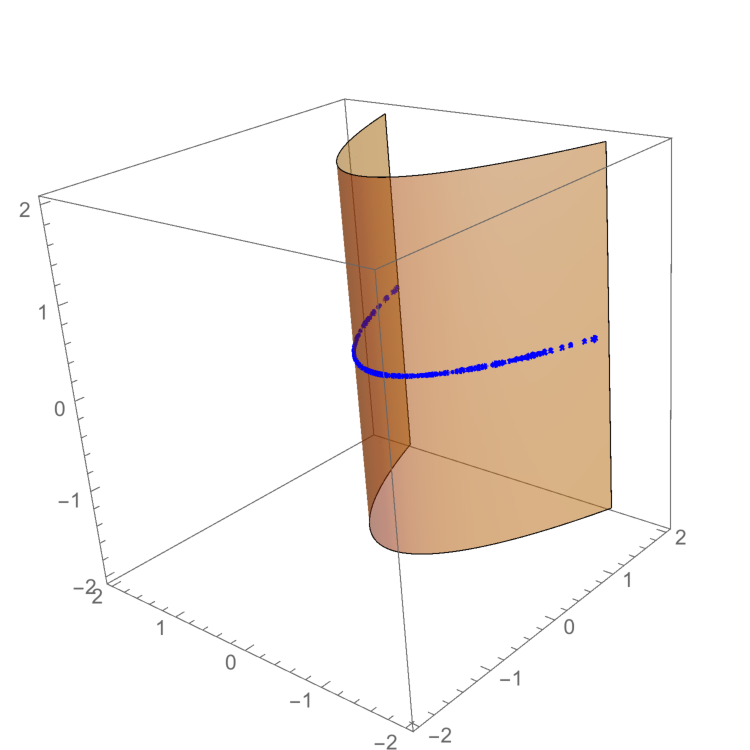
\includegraphics[width=\textwidth]{../pictures/affine_1_exceptional.pdf} 
        \end{subfigure}
        ~
        \begin{subfigure}[t]{0.3\textwidth}
            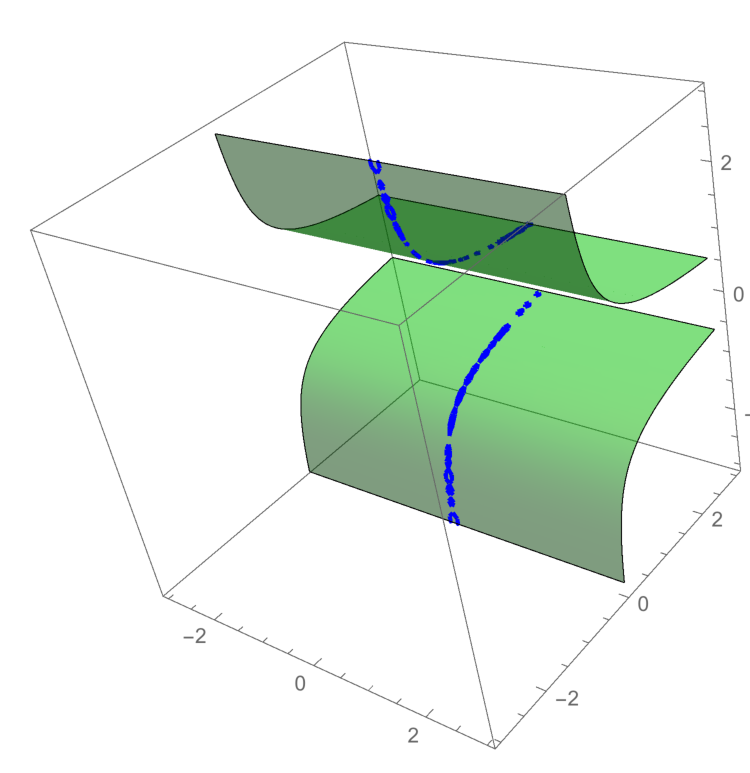
\includegraphics[width=\textwidth]{../pictures/affine_2_exceptional.pdf} 
        \end{subfigure}
        \caption{The two affine charts of the variety $\V(x^2y-z^2)$. The top
            row is rendered by \textsc{Surfer}, and the bottom row rendered by
            \textsc{Mathematica.} The exceptional divisor in the top row has
            been divided out and is therefore not shown because \textsc{Surfer}
        does a poor job at rendering planes. As seen, the charts are smooth and
    exhibits no singularities. The intersection with the exceptional divisor is
rendered in blue in the bottom row.}
    \end{figure}
\end{example}

While in the above example we blew up a very specific line of singularities,
namely the $y$-axis, it can be of interest to talk a little bit about how to
blow up general lines. It all boils down to generalizing the construction of
the plane for a more general line $L$. Assuming $L$ is parametrized by $x = at,
y = bt, z = ct$, with $a, b$ and $c$ non-zero, we can form the symmetric
equations 
\begin{equation}
    \notag
    t = \frac{x}{a} = \frac{y}{b} = \frac{z}{c}.
\end{equation}
The line $L$ is then completely determined by two of the three possible
relations $xb - ya = 0$, $xc - za = 0$ and $yc - zb = 0$.  In order to find the
respective plane, we are interested in knowing when the plane $rx + sy + tz =
0$ can be expressed in terms of the line given by $xb - ya = 0$ and $yc - zb =
0$. This can be solved as a matrix problem. Given the matrix
\begin{equation}
    \notag
    A = \begin{bmatrix}
        b & 0 & r \\
        -a & c & s \\
        0 & -b & t
    \end{bmatrix}
\end{equation}
one of the columns of $A$ is linearly dependent of the two others if $\det(A) =
0$. Solving $\det(A) = 0$ gives the equation
\begin{equation}
    \notag
    \det(A) = b(ct + sb) + rab = 0.
\end{equation}
We can now solve for either one of $r, s$ and $t$. Solving for $r$ we get $r =
-( ct + sb ) / a$ which we can substitute back into the equation for our plane.
The plane is then determined by 
\begin{equation}
    \notag
    \frac{-ct - sb}{a}x + sy + tz = 0.
\end{equation}
Multiplying through by $a$ we achieve
\begin{align*}
    (-sb - ct)x + sya + tza &= -sbx - ctx + sya + tza \\
                            &= t(za - cx) + s(ya - bx) = 0.
\end{align*}
\clearpage
\appendix

\newgeometry{margin=4cm}

\section{Code Samples}
\label{sec:code_samples}

\lstset{deletekeywords={xrange}}
\begin{TMcode}{python}{curves.py - \url{http://stackoverflow.com/a/2484594}}{Plotting algebraic curves}
import matplotlib.pyplot
from numpy import arange
from numpy import meshgrid

delta = 0.025
xrange = arange(-5, 5.0, delta)
yrange = arange(-2.5, 2.5, delta)
X, Y = meshgrid(xrange,yrange)

# F is one side of the equation, G is the other
F = X**2*(1 - Y**2 - X*Y**3)
G = 0

matplotlib.pyplot.axis('on')
matplotlib.pyplot.grid('on')
matplotlib.pyplot.contour(X, Y, (F - G), [0])

matplotlib.pyplot.savefig('output.pdf')
\end{TMcode}

\clearpage
\begin{TMcode}{mathematica}{intersection.nb - \url{http://community.wolfram.com/groups/-/m/t/178218?p_p_auth=lT7er3Rd}}{Plotting the intersection between to surfaces}

(* affine chart and exceptional divisor *)
h = z^2 y - 1;
g = x^2;

ContourPlot3D[
    {h == 0, g == 0}, 
    (* bounding box dimensions *)
    {x, -3, 3}, 
    {y, -3, 3}, 
    {z, -3, 3}, 
    MeshFunctions -> {
        Function[ {x, y, z, f}, h - g ]
    }, 
    MeshStyle -> {
        { Thick, Blue }
    }, 
    Mesh -> {{0}}, 
    ContourStyle -> Directive[
            Green, Opacity[0.5], Specularity[White, 30]
    ], 
    PlotPoints -> 60,
    SphericalRegion -> True
]
\end{TMcode}

\printindex
\end{document}
